\documentclass[a4paper]{article}%

\usepackage[english]{babel}%
\usepackage[utf8]{inputenc}%
\usepackage[T1]{fontenc} %

\usepackage{graphicx}%
\usepackage{xspace}%

\usepackage{amsmath}
\usepackage{amsfonts}
\usepackage{amssymb}

\usepackage[margin=2.5cm]{geometry}

\usepackage{caption}
\usepackage{subcaption}
\usepackage{float}  % H option for figures

\DeclareMathOperator{\E}{E}
\DeclareMathOperator{\Cod}{Cod}
\newcommand{\CodSk}{\overset{\sim}{\Cod}}


\begin{document}

\title{Project IRESI}

\author{Simon Bihel, Florestan De Moor \\ ENS Rennes, Computer Science Department, 1st year}

\date{November 22, 2015}

\maketitle

\begin{abstract}
	In this report we present our work on the project of the course IRESI. We will first explain how we implemented the sketch codeviance, which is a metric used to detect DDoS. We coded this using the Python 3 language. We will then compare the results of the algorithm to exact values.
\end{abstract}


\section{DDoS and server security}
% Simon / Florestan
What's DDoS, difficulty of detecting it, need of distributed algorithm.


\section{Programming the SketchMin algorithm}
% mini intro 2l
For the detection we need to first select the entries to then apply the algorithm that will produce the material in which we will find whether or not there is an attack.

\subsection{Extracting information from data traces}
% Simon
Translate if needed to integers. ??? Could be repetitive with subsection Real data traces.

\subsection{Computing the codeviance}
% Florestan

\paragraph{}First, we implemented two functions to compute the average, and covariance of an array. To do this, we browse the array, and use the following formulas :
	\[ \E(X) = \frac{1}{|X|} \sum\limits_{x_i \in X} x_i \]
	\[ \Cod(X,Y) = \E(XY) - \E(X)\E(Y) \]
	
\paragraph{}We have in entry a data trace $D$, and precision parameters $(\varepsilon, \delta)$. We start by defining the following constants :
	\[ k =\left\lceil \frac{1}{\varepsilon} \right\rceil \]
$k$ is the number of partitions we will create.
	\[ t = \left\lceil \log(\frac{1}{\delta}) \right\rceil \]
$t$ is the number of hashing functions we will consider.
	
\paragraph{}The data trace has integers values which stand between $0$ and $u$. We have to define $t$ universal hashing functions $h_i$ :
	\[ h_i(x) = ((a_ix+b_i) \mod u) \mod k \quad \forall i \in \lbrace 1 \ldots t \rbrace \]
where $a_i, b_i$ are randomly generated in $\lbrace 1 \dots t-1 \rbrace$ for $a_i$, and $\lbrace 0 \ldots t-1 \rbrace$ for $b_i$.

\paragraph{}We can then create the partitions, and we get a matrix $R_{0 \leq i \leq t-1, 1 \leq j \leq k}$ where 
 	\[ R_{i,j} = \# \lbrace x \in D : h_i(x) = j \rbrace \]
 	
\paragraph{}We can now create a function that receive two data traces. It calculates the $D$ matrix for both trace, and then computes the codeviance :
	\[ \CodSk(D_1, D_2) = \underset{0 \leq i \leq t-1}{\min} \Cod(R_1[i], R_2[i]) \]
where $R[i]$ is the line $i$ of the matrix.

\paragraph{}We can then create the full codeviance matrix $C_{1 \leq i,j \leq p}$ when we have $p$ data traces :
	\[ C_{i,j} = \CodSk(D_i, D_j) \quad \forall i,j \in \lbrace 1 \ldots p \rbrace \]
We can notice that the codeviance is symmetrical (i.e. $\Cod(X,Y) = \Cod(Y,X)$). That's why only $p(p+1)/2$ computations are made to create this matrix (instead of $p^2$).

\paragraph{}Once we calculated this matrix, we can plot it in 3D to have a visual result.



\section{Experimental results}
% mini intro 2l
To evaluate the correctness of the algorithm, we just need to see if the results have the same appearance than the real values, with possibly a larger scale.

\subsection{Real data traces}
% Simon
Extracting all at once to maybe find correlation, even after applying the bijection. Extracting the file-names cause the third kind of traces was unusable if we wanted to analyze the sources, as it only says if an internal or external request.


% Just giving the parameters and putting the screenshots

\begin{itemize}
	\item $\varepsilon = 0.001$
	\item $\delta = 0.001$
\end{itemize}

\begin{figure}[!h]
	\center
	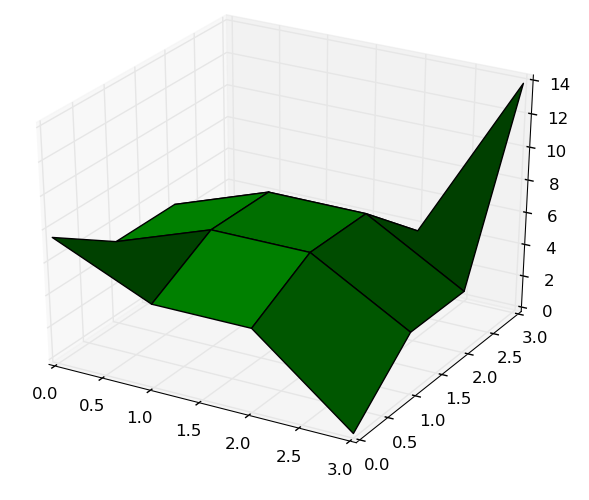
\includegraphics[scale=0.35]{realtests_real1.png}
	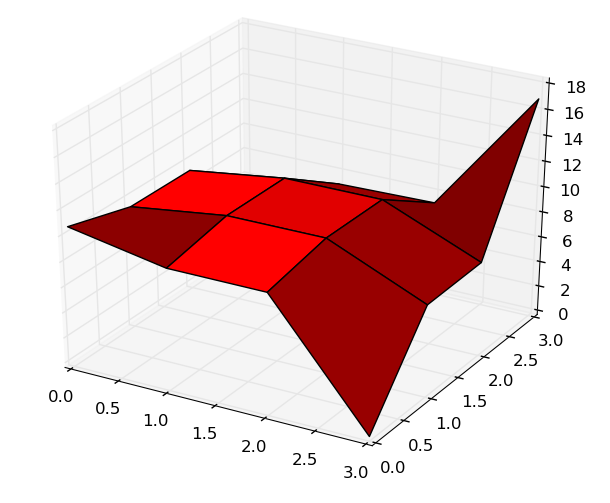
\includegraphics[scale=0.35]{realtests_sketchmin1.png}
	\caption{Codeviance matrix of real data traces: \\real one (green) - calculated with \texttt{SketchMin} algorithm (red)}
\end{figure}


\subsection{Generated data traces}
% Florestan

We generated artificial data traces using some probabilistic laws. Here are the parameters of this experiment :
\begin{itemize}
	\item size of the traces : $size = 10 000$
	\item integers values are generated between $0$ and $u = 100$
	\item $\varepsilon = 0.1$
	\item $\delta = 0.001$
\end{itemize}

\begin{center}
	\begin{tabular}{|c|c|c|}
		\hline
		 & Probabilistic laws & Parameters \\
		 \hline
		Trace 0 & Uniform & \\
		Trace 1 & Zipfian & $\alpha = 2$ \\
		Trace 2 & Zipfian & $\alpha = 3$ \\
		Trace 3 & Zipfian & $\alpha = 4$ \\
		Trace 4 & Zipfian & $\alpha = 5$ \\ 
		Trace 5 & Zipfian & $\alpha = 6$ \\
		Trace 6 & Poisson & $\lambda = u/(2)$ \\
		Trace 7 & Poisson & $\lambda = u/(2^2)$ \\
		Trace 8 & Poisson & $\lambda = u/(2^3)$ \\
		Trace 9 & Poisson & $\lambda = u/(2^4)$ \\
		Trace 10 & Poisson & $\lambda = u/(2^5)$ \\
		Trace 11 & Binomial & $p = 0.42$ \\
		Trace 12 & Negative Binomial & $p = 0.42$ \\
		\hline
	\end{tabular}
\end{center}


We calculated the real codeviance matrix, and we applied the \texttt{SketchMin} algorithm. Here are below the results we got. We can notice that the two shapes are really similar.

\begin{figure}[!h]
	\center
	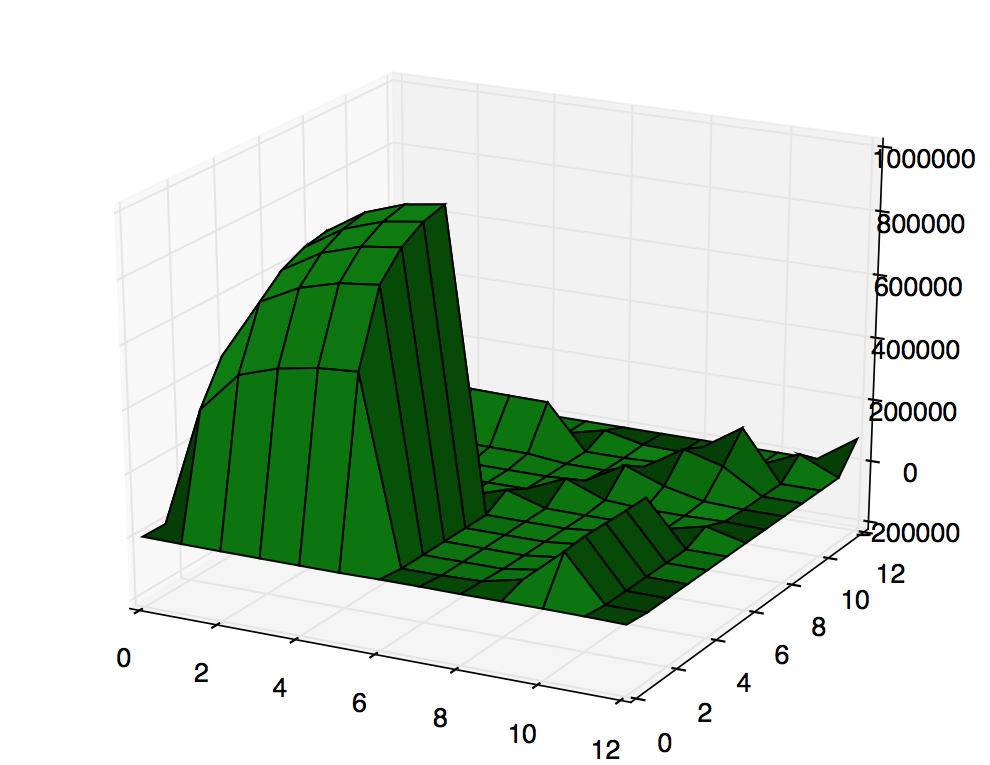
\includegraphics[scale=0.23]{generated_real.png}
	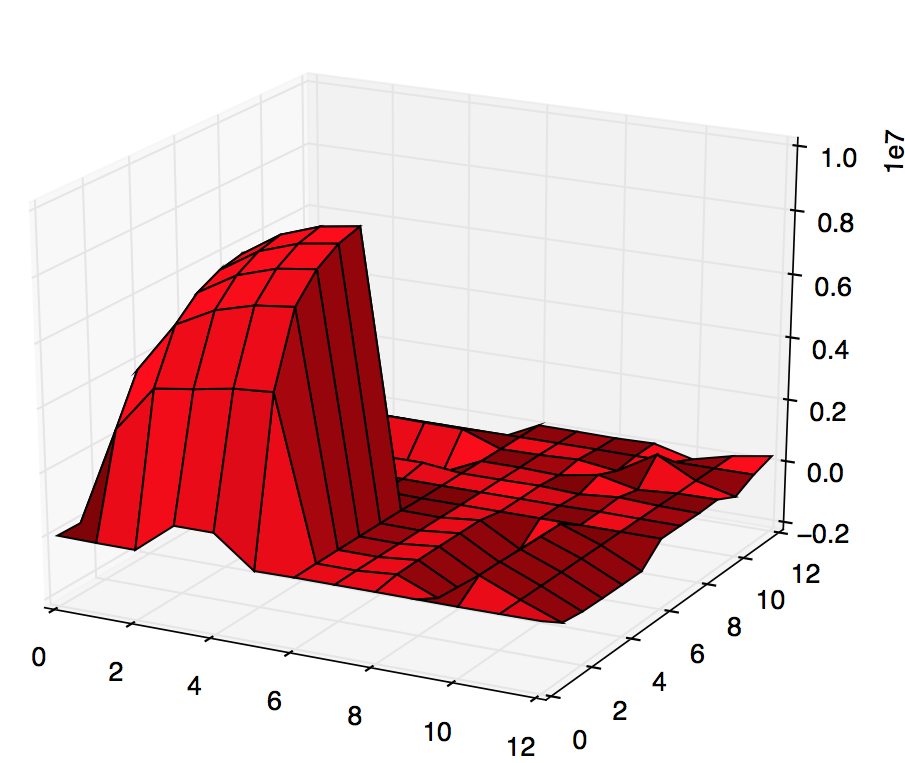
\includegraphics[scale=0.23]{generated_sk.png}
	\caption{Codeviance matrix of generated data traces:\\real one (green) - calculated with \texttt{SketchMin} algorithm (red)}
\end{figure}


\section*{Conclusion}
% Simon / Florestan

\clearpage

\end{document}